
\chapter{Reciprocal (inverse) function}
\competences{finding a domain, differentiating, studying a sign, drawing up a table of variations, graphing}
\section{Reference notes}
The reciprocal function is defined by $f(x)=\dfrac1x$ on $\R\setminus\{0\}$.

\begin{center}
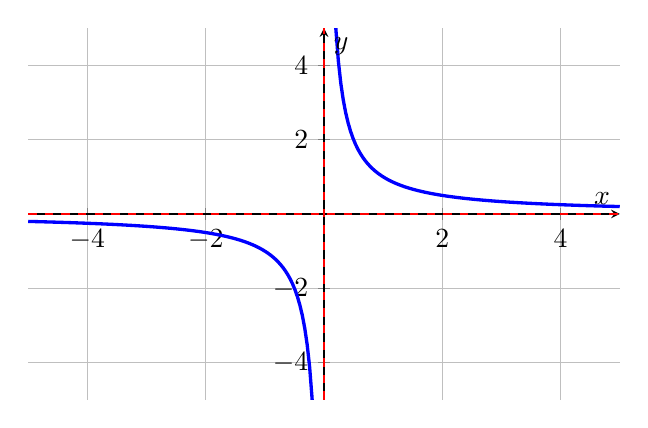
\begin{tikzpicture}
\begin{axis}[width=.75\textwidth,height=6.3cm,axis lines=middle,xmin=-5,xmax=5,ymin=-5,ymax=5,grid=major,xlabel={$x$},ylabel={$y$},unbounded coords=jump]
\addplot[Blue,very thick,samples=120,domain=-5:-.12]{1/x};
\addplot[Blue,very thick,samples=120,domain=.12:5]{1/x};
\addplot[Red,dashed,thick] coordinates {(0,-5)(0,5)};
\addplot[Red,dashed,thick] coordinates {(-5,0)(5,0)};
\end{axis}
\end{tikzpicture}
\end{center}

\begin{retenir}
$f'(x)=-\dfrac1{x^2}<0$ for every $x\neq0$. The reciprocal function is strictly decreasing on each of the intervals $]-\infty,0[$ and $]0,+\infty[$. The lines $x=0$ and $y=0$ are asymptotes.
\end{retenir}

\begin{erreur}
One cannot write that the reciprocal function is decreasing ``on $\R\setminus\{0\}$'' without specifying the two intervals. For example $-1<1$ but $f(-1)=-1<1=f(1)$, which would contradict the global definition of decreasing.
\end{erreur}

For a function $g(x)=P(x)+\dfrac{k}{x}$, proceed in this order: domain; derivative; common denominator and factorisation; sign of the derivative; variations; limits or behaviour at the boundaries; useful points; graph.

\begin{exemple}
On $]0,+\infty[$, $g(x)=x+\dfrac4x$ satisfies $g'(x)=1-\dfrac4{x^2}=\dfrac{(x-2)(x+2)}{x^2}$. The denominator is positive; $g'$ is negative on $]0,2[$ then positive on $]2,+\infty[$. The function has a minimum $g(2)=4$.
\end{exemple}

\sessionheader{23}{15 Dec 2026}{B: 2 h -- C: 1 h}{Definition and graph of the reciprocal function}{Reciprocal (inverse) function}
\begin{objectifs}\begin{itemize}\item Find the domain.\item Draw the curve.\item Use symmetries.\end{itemize}\end{objectifs}
\begin{automatismes}\begin{enumerate}\item Simplify $3x+5-x+2$. \rep{$2x+7$}\item Give the excluded value of $\dfrac{x+1}{x}$. \rep{$x=0$}\item Calculate $\dfrac1{5}$ and $\dfrac1{-5}$. \rep{$\dfrac1{5}$ and $-\dfrac1{5}$}\item Differentiate $3x^2-5x+1$. \rep{$6x-5$}\item Solve $(x-2)(x+1)=0$. \rep{$x=-1$ or $x=2$}\end{enumerate}\end{automatismes}
\begin{prerequis}Reread the last written record and be able to carry out the basic calculations needed today. Before the investigation, have students rephrase the key words: find the domain and draw the curve.\end{prerequis}

\begin{activite}
Calculate $\dfrac1x$ for $x=-4,-2,-1,-\dfrac12,\dfrac12,1,2,4$. Plot the points and describe the symmetries. Why is $x=0$ missing?
\begin{center}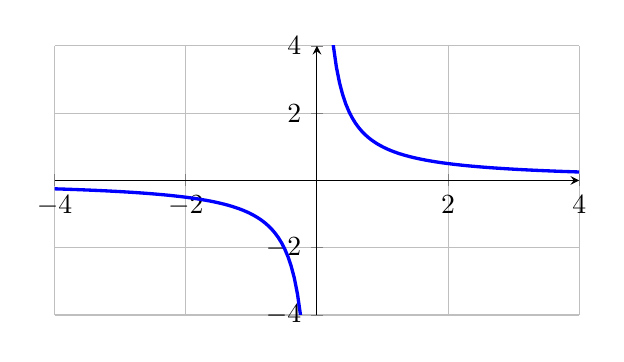
\begin{tikzpicture}\begin{axis}[width=.68\textwidth,height=5cm,axis lines=middle,xmin=-4,xmax=4,ymin=-4,ymax=4,grid=major]\addplot[Blue,very thick,samples=80,domain=-4:-.15]{1/x};\addplot[Blue,very thick,samples=80,domain=.15:4]{1/x};\end{axis}\end{tikzpicture}\end{center}
\end{activite}
\enseignant{The values are respectively $-\frac14,-\frac12,-1,-2,2,1,\frac12,\frac14$. The domain excludes $0$; the curve is symmetric about the origin. Have students say aloud which piece of data triggers the choice of method.}

\begin{traceecrite}The reciprocal function is $f(x)=\dfrac1x$ on $\R\setminus\{0\}$. Its curve is a hyperbola symmetric about the origin.\end{traceecrite}

\begin{exemple}
Revisit the data from the investigation and write up the solution in order: definition of the objects, property used, exact or approximate calculation, then a concluding sentence. The model answer appears in the teacher edition.
\end{exemple}
\enseignant{The values are respectively $-\frac14,-\frac12,-1,-2,2,1,\frac12,\frac14$. The domain excludes $0$; the curve is symmetric about the origin.}

\begin{exercice}[-- essential]
\begin{enumerate}\item Give the domain and the asymptotes of $f(x)=5+\dfrac{7}x$.\item Calculate $f'(x)$ and study its sign.\item Study the function $g(x)=x+\dfrac{25}x$ on $]0,+\infty[$.\end{enumerate}
\end{exercice}
\enseignant{The domain is $\R\setminus\{0\}$; asymptotes $x=0$ and $y=5$. $f'(x)=-\dfrac{7}{x^2}<0$. For $g$, $g'(x)=1-\dfrac{25}{x^2}$ and the minimum is reached at $x=5$, with value $10$.}

\manuelref{Calao, course pp. 88--93; exercises p. 94, no.~1--5}
\CalaoSession{23}

\begin{dm}Redo practice exercise 2 with the following data: replace the initial value by $235$ and the rate or common ratio by $7$. Write it up in four lines: data, formula, calculation, conclusion.\end{dm}
\enseignant{The answer depends on the exercise revisited. Check above all the consistency of the model, the number of iterations, the rounding and the concluding sentence.}

\begin{sortie}On a half-sheet: write the main rule of the session, work through a very short example and state your confidence level from 1 to 4. Key question(s) of the day: 1, 2 and 3.\end{sortie}

\ifprof
\begin{methode}
\textbf{1 h session:} 7 min of fluency; 10 min of pooling and written record; 28 min of essential exercises; 5 min of correction; 3 min of exit ticket.\\
\textbf{2 h session:} add 20 min of investigation, 20 min of formalisation, a second independent exercise and 10 min of comparative correction.\\
\textbf{Differentiation:} give struggling students a four-box sheet (data, model, calculation, conclusion). Ask quick students to produce a counterexample, a justification or a second method.
\end{methode}
\fi
\sessionheader{24}{17 Dec 2026}{B: 1 h -- C: 2 h}{Behaviour at the boundaries and asymptotes}{Reciprocal (inverse) function}
\begin{objectifs}\begin{itemize}\item Describe the behaviour at the boundaries.\item Identify the asymptotes.\item Read a graph.\end{itemize}\end{objectifs}
\begin{automatismes}\begin{enumerate}\item Calculate $5\,\%$ of $120$. \rep{$6$}\item Calculate $\dfrac1{6}$ and $\dfrac1{-6}$. \rep{$\dfrac1{6}$ and $-\dfrac1{6}$}\item Differentiate $3x^2-5x+1$. \rep{$6x-5$}\item Solve $(x-2)(x+1)=0$. \rep{$x=-1$ or $x=2$}\item Give the excluded value of $\dfrac{x+1}{x}$. \rep{$x=0$}\end{enumerate}\end{automatismes}
\begin{prerequis}Reread the last written record and be able to carry out the basic calculations needed today. Before the investigation, have students rephrase the key words: describe the behaviour at the boundaries and identify the asymptotes.\end{prerequis}

\begin{activite}
Using a table of values near $0$ and for large values of $|x|$, describe $\dfrac1x$. Translate each behaviour into an asymptote and a sentence.
\begin{center}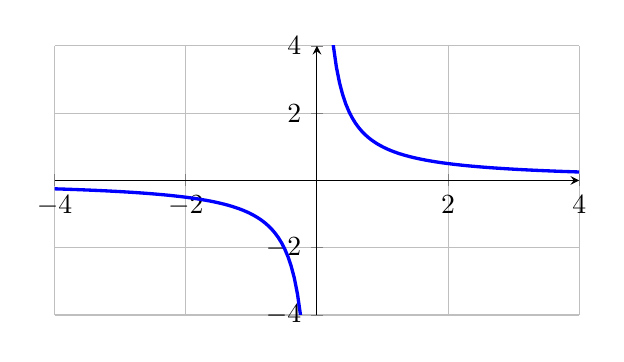
\begin{tikzpicture}\begin{axis}[width=.68\textwidth,height=5cm,axis lines=middle,xmin=-4,xmax=4,ymin=-4,ymax=4,grid=major]\addplot[Blue,very thick,samples=80,domain=-4:-.15]{1/x};\addplot[Blue,very thick,samples=80,domain=.15:4]{1/x};\end{axis}\end{tikzpicture}\end{center}
\end{activite}
\enseignant{Near $0$, the values become very large in absolute value: asymptote $x=0$. As $|x|$ grows, $\dfrac1x$ gets closer to $0$: asymptote $y=0$. Have students say aloud which piece of data triggers the choice of method.}

\begin{traceecrite}For $f(x)=\dfrac1x$, $x=0$ is a vertical asymptote and $y=0$ a horizontal asymptote. The branches approach them without crossing them.\end{traceecrite}

\begin{exemple}
Revisit the data from the investigation and write up the solution in order: definition of the objects, property used, exact or approximate calculation, then a concluding sentence. The model answer appears in the teacher edition.
\end{exemple}
\enseignant{Near $0$, the values become very large in absolute value: asymptote $x=0$. As $|x|$ grows, $\dfrac1x$ gets closer to $0$: asymptote $y=0$.}

\begin{exercice}[-- essential]
\begin{enumerate}\item Give the domain and the asymptotes of $f(x)=6+\dfrac{8}x$.\item Calculate $f'(x)$ and study its sign.\item Study the function $g(x)=x+\dfrac{36}x$ on $]0,+\infty[$.\end{enumerate}
\end{exercice}
\enseignant{The domain is $\R\setminus\{0\}$; asymptotes $x=0$ and $y=6$. $f'(x)=-\dfrac{8}{x^2}<0$. For $g$, $g'(x)=1-\dfrac{36}{x^2}$ and the minimum is reached at $x=6$, with value $12$.}

\manuelref{Calao, course pp. 88--93; exercises p. 94, no.~4--9}
\CalaoSession{24}

\begin{dm}Redo practice exercise 3 with the following data: replace the initial value by $240$ and the rate or common ratio by $2$. Write it up in four lines: data, formula, calculation, conclusion.\end{dm}
\enseignant{The answer depends on the exercise revisited. Check above all the consistency of the model, the number of iterations, the rounding and the concluding sentence.}

\begin{sortie}On a half-sheet: write the main rule of the session, work through a very short example and state your confidence level from 1 to 4. Key question(s) of the day: 1 and 2.\end{sortie}

\ifprof
\begin{methode}
\textbf{1 h session:} 7 min of fluency; 10 min of pooling and written record; 28 min of essential exercises; 5 min of correction; 3 min of exit ticket.\\
\textbf{2 h session:} add 20 min of investigation, 20 min of formalisation, a second independent exercise and 10 min of comparative correction.\\
\textbf{Differentiation:} give struggling students a four-box sheet (data, model, calculation, conclusion). Ask quick students to produce a counterexample, a justification or a second method.
\end{methode}
\fi
\sessionheader{25}{5 Jan 2027}{B: 2 h -- C: 1 h}{Derivative and direction of variation}{Reciprocal (inverse) function}
\begin{objectifs}\begin{itemize}\item Differentiate the reciprocal function.\item Justify the variations.\item Draw up a table.\end{itemize}\end{objectifs}
\begin{automatismes}\begin{enumerate}\item Write the multiplier for an increase of $10\,\%$. \rep{$1+\dfrac{10}{100}=1.10$}\item Differentiate $3x^2-5x+1$. \rep{$6x-5$}\item Solve $(x-2)(x+1)=0$. \rep{$x=-1$ or $x=2$}\item Give the excluded value of $\dfrac{x+1}{x}$. \rep{$x=0$}\item Calculate $\dfrac1{7}$ and $\dfrac1{-7}$. \rep{$\dfrac1{7}$ and $-\dfrac1{7}$}\end{enumerate}\end{automatismes}
\begin{prerequis}Reread the last written record and be able to carry out the basic calculations needed today. Before the investigation, have students rephrase the key words: differentiate the reciprocal function and justify the variations.\end{prerequis}

\begin{activite}
Starting from the difference quotient of $f(x)=\dfrac1x$, recover $f'(x)=-\dfrac1{x^2}$. Study its sign and check consistency with the graph.

\end{activite}
\enseignant{The square $x^2$ is positive for $x\neq0$, so the derivative is strictly negative on each interval of the domain. Have students say aloud which piece of data triggers the choice of method.}

\begin{traceecrite}For $x\neq0$, $f'(x)=-\dfrac1{x^2}<0$. The reciprocal function decreases on each of the intervals $]-\infty,0[$ and $]0,+\infty[$.\end{traceecrite}

\begin{exemple}
Revisit the data from the investigation and write up the solution in order: definition of the objects, property used, exact or approximate calculation, then a concluding sentence. The model answer appears in the teacher edition.
\end{exemple}
\enseignant{The square $x^2$ is positive for $x\neq0$, so the derivative is strictly negative on each interval of the domain.}

\begin{exercice}[-- essential]
\begin{enumerate}\item Give the domain and the asymptotes of $f(x)=2+\dfrac{4}x$.\item Calculate $f'(x)$ and study its sign.\item Study the function $g(x)=x+\dfrac{4}x$ on $]0,+\infty[$.\end{enumerate}
\end{exercice}
\enseignant{The domain is $\R\setminus\{0\}$; asymptotes $x=0$ and $y=2$. $f'(x)=-\dfrac{4}{x^2}<0$. For $g$, $g'(x)=1-\dfrac{4}{x^2}$ and the minimum is reached at $x=2$, with value $4$.}

\manuelref{Calao, course pp. 89--93; exercises p. 94, no.~1--3, then p. 96, no.~10--13}
\CalaoSession{25}

\begin{dm}Redo practice exercise 2 with the following data: replace the initial value by $245$ and the rate or common ratio by $3$. Write it up in four lines: data, formula, calculation, conclusion.\end{dm}
\enseignant{The answer depends on the exercise revisited. Check above all the consistency of the model, the number of iterations, the rounding and the concluding sentence.}

\begin{sortie}On a half-sheet: write the main rule of the session, work through a very short example and state your confidence level from 1 to 4. Key question(s) of the day: 1, 2 and 3.\end{sortie}

\ifprof
\begin{methode}
\textbf{1 h session:} 7 min of fluency; 10 min of pooling and written record; 28 min of essential exercises; 5 min of correction; 3 min of exit ticket.\\
\textbf{2 h session:} add 20 min of investigation, 20 min of formalisation, a second independent exercise and 10 min of comparative correction.\\
\textbf{Differentiation:} give struggling students a four-box sheet (data, model, calculation, conclusion). Ask quick students to produce a counterexample, a justification or a second method.
\end{methode}
\fi
\sessionheader{26}{7 Jan 2027}{B: 1 h -- C: 2 h}{Combinations with polynomial functions}{Reciprocal (inverse) function}
\begin{objectifs}\begin{itemize}\item Differentiate a combination of functions.\item Simplify an expression.\item Organise a function study.\end{itemize}\end{objectifs}
\begin{automatismes}\begin{enumerate}\item Simplify $3x+8-x+2$. \rep{$2x+10$}\item Solve $(x-2)(x+1)=0$. \rep{$x=-1$ or $x=2$}\item Give the excluded value of $\dfrac{x+1}{x}$. \rep{$x=0$}\item Calculate $\dfrac1{8}$ and $\dfrac1{-8}$. \rep{$\dfrac1{8}$ and $-\dfrac1{8}$}\item Differentiate $3x^2-5x+1$. \rep{$6x-5$}\end{enumerate}\end{automatismes}
\begin{prerequis}Reread the last written record and be able to carry out the basic calculations needed today. Before the investigation, have students rephrase the key words: differentiate a combination of functions and simplify an expression.\end{prerequis}

\begin{activite}
A company produces $x>0$ hundred items and its average cost is $C(x)=2x+30+\dfrac{200}{x}$. Calculate $C'(x)$, factorise its numerator and find the production level that minimises the average cost.

\end{activite}
\enseignant{$C'(x)=2-\dfrac{200}{x^2}=\dfrac{2(x-10)(x+10)}{x^2}$. The minimum is reached for $x=10$, that is $1\,000$ items. Have students say aloud which piece of data triggers the choice of method.}

\begin{traceecrite}To study $P(x)+\dfrac{k}{x}$, find the domain, calculate the derivative, put over a common denominator, study its sign, then draw up the variations.\end{traceecrite}

\begin{exemple}
Revisit the data from the investigation and write up the solution in order: definition of the objects, property used, exact or approximate calculation, then a concluding sentence. The model answer appears in the teacher edition.
\end{exemple}
\enseignant{$C'(x)=2-\dfrac{200}{x^2}=\dfrac{2(x-10)(x+10)}{x^2}$. The minimum is reached for $x=10$, that is $1\,000$ items.}

\begin{exercice}[-- essential]
\begin{enumerate}\item Give the domain and the asymptotes of $f(x)=3+\dfrac{5}x$.\item Calculate $f'(x)$ and study its sign.\item Study the function $g(x)=x+\dfrac{9}x$ on $]0,+\infty[$.\end{enumerate}
\end{exercice}
\enseignant{The domain is $\R\setminus\{0\}$; asymptotes $x=0$ and $y=3$. $f'(x)=-\dfrac{5}{x^2}<0$. For $g$, $g'(x)=1-\dfrac{9}{x^2}$ and the minimum is reached at $x=3$, with value $6$.}

\manuelref{Calao, p. 96, no.~14--21}
\CalaoSession{26}

\begin{dm}Redo practice exercise 3 with the following data: replace the initial value by $250$ and the rate or common ratio by $4$. Write it up in four lines: data, formula, calculation, conclusion.\end{dm}
\enseignant{The answer depends on the exercise revisited. Check above all the consistency of the model, the number of iterations, the rounding and the concluding sentence.}

\begin{sortie}On a half-sheet: write the main rule of the session, work through a very short example and state your confidence level from 1 to 4. Key question(s) of the day: 1 and 2.\end{sortie}

\ifprof
\begin{methode}
\textbf{1 h session:} 7 min of fluency; 10 min of pooling and written record; 28 min of essential exercises; 5 min of correction; 3 min of exit ticket.\\
\textbf{2 h session:} add 20 min of investigation, 20 min of formalisation, a second independent exercise and 10 min of comparative correction.\\
\textbf{Differentiation:} give struggling students a four-box sheet (data, model, calculation, conclusion). Ask quick students to produce a counterexample, a justification or a second method.
\end{methode}
\fi
\sessionheader{27}{12 Jan 2027}{B: 2 h -- C: 1 h}{Sign and factorisation}{Reciprocal (inverse) function}
\begin{objectifs}\begin{itemize}\item Factorise.\item Build a sign table.\item Respect excluded values.\end{itemize}\end{objectifs}
\begin{automatismes}\begin{enumerate}\item Calculate $20\,\%$ of $180$. \rep{$36$}\item Give the excluded value of $\dfrac{x+1}{x}$. \rep{$x=0$}\item Calculate $\dfrac1{9}$ and $\dfrac1{-9}$. \rep{$\dfrac1{9}$ and $-\dfrac1{9}$}\item Differentiate $3x^2-5x+1$. \rep{$6x-5$}\item Solve $(x-2)(x+1)=0$. \rep{$x=-1$ or $x=2$}\end{enumerate}\end{automatismes}
\begin{prerequis}Reread the last written record and be able to carry out the basic calculations needed today. Before the investigation, have students rephrase the key words: factorise and build a sign table.\end{prerequis}

\begin{activite}
Study the sign of $\dfrac{(x-2)(x+3)}x$. Build the table with the three critical values, distinguish a zero from an excluded value, then solve the inequality $\dfrac{(x-2)(x+3)}x\geq0$.

\end{activite}
\enseignant{The critical values are $-3,0,2$. The solution is $[-3,0[\cup[2,+\infty[$. Have students say aloud which piece of data triggers the choice of method.}

\begin{traceecrite}In a quotient, the sign depends on the numerator and the denominator. Excluded values are left out of the table, even if a factor formally cancels.\end{traceecrite}

\begin{exemple}
Revisit the data from the investigation and write up the solution in order: definition of the objects, property used, exact or approximate calculation, then a concluding sentence. The model answer appears in the teacher edition.
\end{exemple}
\enseignant{The critical values are $-3,0,2$. The solution is $[-3,0[\cup[2,+\infty[$.}

\begin{exercice}[-- essential]
\begin{enumerate}\item Give the domain and the asymptotes of $f(x)=4+\dfrac{6}x$.\item Calculate $f'(x)$ and study its sign.\item Study the function $g(x)=x+\dfrac{16}x$ on $]0,+\infty[$.\end{enumerate}
\end{exercice}
\enseignant{The domain is $\R\setminus\{0\}$; asymptotes $x=0$ and $y=4$. $f'(x)=-\dfrac{6}{x^2}<0$. For $g$, $g'(x)=1-\dfrac{16}{x^2}$ and the minimum is reached at $x=4$, with value $8$.}

\manuelref{Calao, pp. 96--101}
\CalaoSession{27}

\begin{dm}Redo practice exercise 2 with the following data: replace the initial value by $255$ and the rate or common ratio by $5$. Write it up in four lines: data, formula, calculation, conclusion.\end{dm}
\enseignant{The answer depends on the exercise revisited. Check above all the consistency of the model, the number of iterations, the rounding and the concluding sentence.}

\begin{sortie}On a half-sheet: write the main rule of the session, work through a very short example and state your confidence level from 1 to 4. Key question(s) of the day: 1, 2 and 3.\end{sortie}

\ifprof
\begin{methode}
\textbf{1 h session:} 7 min of fluency; 10 min of pooling and written record; 28 min of essential exercises; 5 min of correction; 3 min of exit ticket.\\
\textbf{2 h session:} add 20 min of investigation, 20 min of formalisation, a second independent exercise and 10 min of comparative correction.\\
\textbf{Differentiation:} give struggling students a four-box sheet (data, model, calculation, conclusion). Ask quick students to produce a counterexample, a justification or a second method.
\end{methode}
\fi
\sessionheader{28}{14 Jan 2027}{B: 1 h -- C: 2 h}{Derivatives of polynomials of degree at most 3}{Reciprocal (inverse) function}
\begin{objectifs}\begin{itemize}\item Differentiate a polynomial.\item Study a derivative.\item Deduce the variations.\end{itemize}\end{objectifs}
\begin{automatismes}\begin{enumerate}\item Write the multiplier for an increase of $25\,\%$. \rep{$1+\dfrac{25}{100}=1.25$}\item Calculate $\dfrac1{3}$ and $\dfrac1{-3}$. \rep{$\dfrac1{3}$ and $-\dfrac1{3}$}\item Differentiate $3x^2-5x+1$. \rep{$6x-5$}\item Solve $(x-2)(x+1)=0$. \rep{$x=-1$ or $x=2$}\item Give the excluded value of $\dfrac{x+1}{x}$. \rep{$x=0$}\end{enumerate}\end{automatismes}
\begin{prerequis}Reread the last written record and be able to carry out the basic calculations needed today. Before the investigation, have students rephrase the key words: differentiate a polynomial and study a derivative.\end{prerequis}

\begin{activite}
For $f(x)=2x^3-3x^2-12x+5$, calculate $f'(x)$, factorise, study its sign and deduce the variations of $f$.

\end{activite}
\enseignant{$f'(x)=6x^2-6x-12=6(x-2)(x+1)$. The function increases on $]-\infty,-1]$, decreases on $[-1,2]$, then increases. Have students say aloud which piece of data triggers the choice of method.}

\begin{traceecrite}$(ax^3+bx^2+cx+d)'=3ax^2+2bx+c$. The sign of the derivative gives the direction of variation of the function.\end{traceecrite}

\begin{exemple}
Revisit the data from the investigation and write up the solution in order: definition of the objects, property used, exact or approximate calculation, then a concluding sentence. The model answer appears in the teacher edition.
\end{exemple}
\enseignant{$f'(x)=6x^2-6x-12=6(x-2)(x+1)$. The function increases on $]-\infty,-1]$, decreases on $[-1,2]$, then increases.}

\begin{exercice}[-- essential]
\begin{enumerate}\item Give the domain and the asymptotes of $f(x)=5+\dfrac{7}x$.\item Calculate $f'(x)$ and study its sign.\item Study the function $g(x)=x+\dfrac{25}x$ on $]0,+\infty[$.\end{enumerate}
\end{exercice}
\enseignant{The domain is $\R\setminus\{0\}$; asymptotes $x=0$ and $y=5$. $f'(x)=-\dfrac{7}{x^2}<0$. For $g$, $g'(x)=1-\dfrac{25}{x^2}$ and the minimum is reached at $x=5$, with value $10$.}

\manuelref{Calao, pp. 94--96}
\CalaoSession{28}

\begin{dm}Redo practice exercise 3 with the following data: replace the initial value by $260$ and the rate or common ratio by $6$. Write it up in four lines: data, formula, calculation, conclusion.\end{dm}
\enseignant{The answer depends on the exercise revisited. Check above all the consistency of the model, the number of iterations, the rounding and the concluding sentence.}

\begin{sortie}On a half-sheet: write the main rule of the session, work through a very short example and state your confidence level from 1 to 4. Key question(s) of the day: 1 and 2.\end{sortie}

\ifprof
\begin{methode}
\textbf{1 h session:} 7 min of fluency; 10 min of pooling and written record; 28 min of essential exercises; 5 min of correction; 3 min of exit ticket.\\
\textbf{2 h session:} add 20 min of investigation, 20 min of formalisation, a second independent exercise and 10 min of comparative correction.\\
\textbf{Differentiation:} give struggling students a four-box sheet (data, model, calculation, conclusion). Ask quick students to produce a counterexample, a justification or a second method.
\end{methode}
\fi
\sessionheader{29}{19 Jan 2027}{B: 2 h -- C: 1 h}{Full study and graph}{Reciprocal (inverse) function}
\begin{objectifs}\begin{itemize}\item Carry out a full study.\item Draw a consistent curve.\item Interpret an extremum.\end{itemize}\end{objectifs}
\begin{automatismes}\begin{enumerate}\item Simplify $3x+4-x+2$. \rep{$2x+6$}\item Differentiate $3x^2-5x+1$. \rep{$6x-5$}\item Solve $(x-2)(x+1)=0$. \rep{$x=-1$ or $x=2$}\item Give the excluded value of $\dfrac{x+1}{x}$. \rep{$x=0$}\item Calculate $\dfrac1{4}$ and $\dfrac1{-4}$. \rep{$\dfrac1{4}$ and $-\dfrac1{4}$}\end{enumerate}\end{automatismes}
\begin{prerequis}Reread the last written record and be able to carry out the basic calculations needed today. Before the investigation, have students rephrase the key words: carry out a full study and draw a consistent curve.\end{prerequis}

\begin{activite}
Study $g(x)=x+\dfrac9x$ completely on $]0,+\infty[$: domain, derivative, sign, variations, minimum, behaviour at the boundaries and sketch.
\begin{center}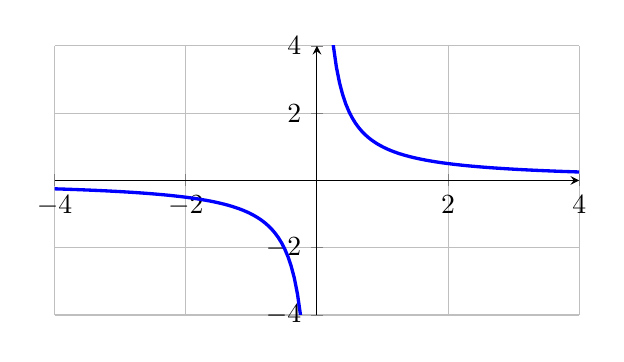
\begin{tikzpicture}\begin{axis}[width=.68\textwidth,height=5cm,axis lines=middle,xmin=-4,xmax=4,ymin=-4,ymax=4,grid=major]\addplot[Blue,very thick,samples=80,domain=-4:-.15]{1/x};\addplot[Blue,very thick,samples=80,domain=.15:4]{1/x};\end{axis}\end{tikzpicture}\end{center}
\end{activite}
\enseignant{$g'(x)=\dfrac{(x-3)(x+3)}{x^2}$; minimum $g(3)=6$; $g(x)$ tends to $+\infty$ at $0^+$ and at $+\infty$. Have students say aloud which piece of data triggers the choice of method.}

\begin{traceecrite}A full study includes: domain, derivative, sign, variations, limits or behaviour at the boundaries, key points and a consistent graph.\end{traceecrite}

\begin{exemple}
Revisit the data from the investigation and write up the solution in order: definition of the objects, property used, exact or approximate calculation, then a concluding sentence. The model answer appears in the teacher edition.
\end{exemple}
\enseignant{$g'(x)=\dfrac{(x-3)(x+3)}{x^2}$; minimum $g(3)=6$; $g(x)$ tends to $+\infty$ at $0^+$ and at $+\infty$.}

\begin{exercice}[-- essential]
\begin{enumerate}\item Give the domain and the asymptotes of $f(x)=6+\dfrac{8}x$.\item Calculate $f'(x)$ and study its sign.\item Study the function $g(x)=x+\dfrac{36}x$ on $]0,+\infty[$.\end{enumerate}
\end{exercice}
\enseignant{The domain is $\R\setminus\{0\}$; asymptotes $x=0$ and $y=6$. $f'(x)=-\dfrac{8}{x^2}<0$. For $g$, $g'(x)=1-\dfrac{36}{x^2}$ and the minimum is reached at $x=6$, with value $12$.}

\manuelref{Calao, pp. 98--103}
\CalaoSession{29}

\begin{dm}Redo practice exercise 2 with the following data: replace the initial value by $265$ and the rate or common ratio by $7$. Write it up in four lines: data, formula, calculation, conclusion.\end{dm}
\enseignant{The answer depends on the exercise revisited. Check above all the consistency of the model, the number of iterations, the rounding and the concluding sentence.}

\begin{sortie}On a half-sheet: write the main rule of the session, work through a very short example and state your confidence level from 1 to 4. Key question(s) of the day: 1, 2 and 3.\end{sortie}

\ifprof
\begin{methode}
\textbf{1 h session:} 7 min of fluency; 10 min of pooling and written record; 28 min of essential exercises; 5 min of correction; 3 min of exit ticket.\\
\textbf{2 h session:} add 20 min of investigation, 20 min of formalisation, a second independent exercise and 10 min of comparative correction.\\
\textbf{Differentiation:} give struggling students a four-box sheet (data, model, calculation, conclusion). Ask quick students to produce a counterexample, a justification or a second method.
\end{methode}
\fi
\sessionheader{30}{21 Jan 2027}{B: 1 h -- C: 2 h}{Review and assessment}{Reciprocal (inverse) function}
\begin{objectifs}\begin{itemize}\item Use domain, derivative and sign.\item Write up a study.\item Correct work methodically.\end{itemize}\end{objectifs}
\begin{automatismes}\begin{enumerate}\item Calculate $5\,\%$ of $100$. \rep{$5$}\item Solve $(x-2)(x+1)=0$. \rep{$x=-1$ or $x=2$}\item Give the excluded value of $\dfrac{x+1}{x}$. \rep{$x=0$}\item Calculate $\dfrac1{5}$ and $\dfrac1{-5}$. \rep{$\dfrac1{5}$ and $-\dfrac1{5}$}\item Differentiate $3x^2-5x+1$. \rep{$6x-5$}\end{enumerate}\end{automatismes}
\begin{prerequis}Reread the last written record and be able to carry out the basic calculations needed today. Before the investigation, have students rephrase the key words: use domain, derivative and sign and write up a study.\end{prerequis}

\begin{activite}
Correct a deliberately flawed study of $h(x)=x+\dfrac4x$: stated domain $\R$, derivative $1+\dfrac4{x^2}$, table with no break at $0$. Rewrite a complete solution.

\end{activite}
\enseignant{The domain is $\R\setminus\{0\}$ and $h'(x)=1-\dfrac4{x^2}$. The table is split at $0$ and takes into account $-2$ and $2$. Have students say aloud which piece of data triggers the choice of method.}

\begin{traceecrite}Check the four items separately: domain, expression of the derivative, sign of the derivative, variations. An error at one step must not hide the following ones.\end{traceecrite}

\begin{exemple}
Revisit the data from the investigation and write up the solution in order: definition of the objects, property used, exact or approximate calculation, then a concluding sentence. The model answer appears in the teacher edition.
\end{exemple}
\enseignant{The domain is $\R\setminus\{0\}$ and $h'(x)=1-\dfrac4{x^2}$. The table is split at $0$ and takes into account $-2$ and $2$.}

\begin{exercice}[-- essential]
\begin{enumerate}\item Give the domain and the asymptotes of $f(x)=2+\dfrac{4}x$.\item Calculate $f'(x)$ and study its sign.\item Study the function $g(x)=x+\dfrac{4}x$ on $]0,+\infty[$.\end{enumerate}
\end{exercice}
\enseignant{The domain is $\R\setminus\{0\}$; asymptotes $x=0$ and $y=2$. $f'(x)=-\dfrac{4}{x^2}<0$. For $g$, $g'(x)=1-\dfrac{4}{x^2}$ and the minimum is reached at $x=2$, with value $4$.}

\manuelref{Calao, pp. 100--103}
\CalaoSession{30}

\begin{dm}Redo practice exercise 3 with the following data: replace the initial value by $270$ and the rate or common ratio by $2$. Write it up in four lines: data, formula, calculation, conclusion.\end{dm}
\enseignant{The answer depends on the exercise revisited. Check above all the consistency of the model, the number of iterations, the rounding and the concluding sentence.}

\begin{sortie}On a half-sheet: write the main rule of the session, work through a very short example and state your confidence level from 1 to 4. Key question(s) of the day: 1 and 2.\end{sortie}

\ifprof
\begin{methode}
\textbf{1 h session:} 7 min of fluency; 10 min of pooling and written record; 28 min of essential exercises; 5 min of correction; 3 min of exit ticket.\\
\textbf{2 h session:} add 20 min of investigation, 20 min of formalisation, a second independent exercise and 10 min of comparative correction.\\
\textbf{Differentiation:} give struggling students a four-box sheet (data, model, calculation, conclusion). Ask quick students to produce a counterexample, a justification or a second method.
\end{methode}
\fi
